\documentclass[jou]{apa6}   %Utilizamos Apa6 mas actualizada, de tipo jorunal.
\usepackage[utf8]{inputenc}       	%Encoding de Utf-8, por compatibilidad con mi vim.
%\usepackage[spanish]{babel} 		%Idioma utilizado para todo el articulo.Toca redefinir
\usepackage{natbib}
\usepackage{subfigure} 				%subfiguras
\usepackage{graphicx}				%Necesario para el manejo de imagenes en el articulo.

\DeclareGraphicsExtensions{.png,.jpg} %Extensiones Soportadas para las imagenes.
%Las imagenes se encuentran en directorio de /images/, mas info en https://en.wikibooks.org/wiki/LaTeX/Importing_Graphics

\title{Descubriendo Controladores Lógicos Programables en una Red Universitaria} 
\shorttitle{ Descubriendo PLC's en una Red Universitaria}

\twoauthors{Héctor Fabio Jiménez Saldarriaga}{Sebastian Zapata Ruiz}
\twoaffiliations{Universidad Tecnológica de Pereira, \\ Ingeniería de Sistemas y Computación, \\Pereira Security Team }{Universidad Tecnológica de Pereira, \\ Ingeniería de Sistemas y Computación}
\keywords{Redes Industriales , Seguridad Informática, Controladores Lógicos}
\abstract{El uso de los dispositivos electrónicos como los controladores lógicos programables  en el campo de la automatización y el control de procesos tienen un rol importante, estos se implementan en muchos campos, e industrias donde los procesos de producción y  administración son complicados,  críticos y peligrosos tanto económicamente como para la vida humana.  En este artículo evidenciamos cómo es posible realizar el descubrimiento de estos dispositivos en un entorno controlado que presenta múltiples PLC's, Computadores de Monitoreo corriendo bajo sistemas operativos Windows, en un	a infraestructura universitaria.}
\leftheader{Hector F. Jimenez S., Sebastian Zapata R.} %Header en la parte superior.

\begin{document}
\maketitle    
                     
\section{Introducción}
Los controladores lógicos programables (\textit{Programmable logic controller}, de ahora en adelante PLC) fueron diseños en los años 60s[Ref1, Segovia] cuando el control de las maquinas industriales se hacía mediante el uso de relés como en la figura (\ref{fig:horizonte}), en ese entonces era tedioso y complicado para un técnico encontrar una falla en el sistema eléctrico de control debido a que todo los procesos se encontraban en cuartos llenos de  una gran cantidad de cables y relés, lo que dificultaba la búsqueda. Con la llegada de los  PLCs se resolvió el problema de la flexibilidad y solución de problemas comunes; estos reemplazaron decenas de cuartos en pocos, albergando bloques compactos de PLC, con ventajas como fácil mantenimiento, instalación, expansión. Su labor principal es la regulación  los actuadores electromecánicos, como pueden ser válvulas, sensores, bombas, motores, etc.\\

\begin{figure}[htb]
\centering
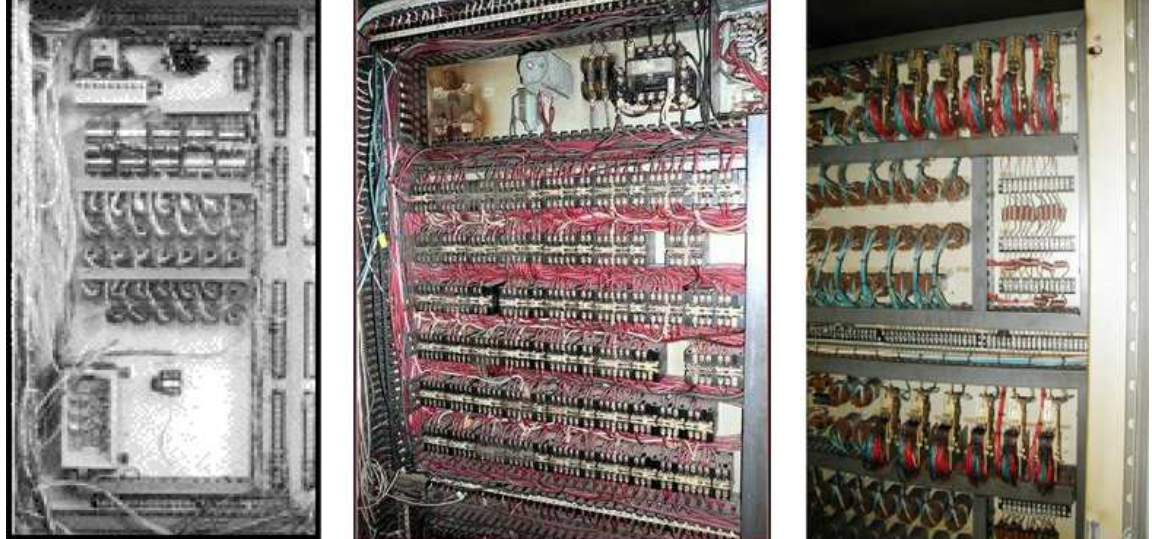
\includegraphics[scale=0.2]{images/relayroom.png}
\caption{Cuarto de Control Reles, 1974.} \label{fig:horizonte}
\end{figure}

Los sistemas de control utilizan como uno de los componentes a los PLCs  para regular procesos industriales  ejemplos de estas tareas de producción química, líneas de ensamblaje y manufactura, maniobra de maquinaria pesada,  control y manejo de señales, control de mezclas, control de generación y despacho eléctrico entre otros. En un principio de estos dispositivos se presenta cada PLC como controlador individual e independiente, pero con el crecimiento y demanda de los procesos se requería  tener conexiones con otros PLCs, lo cual solo funcionaba en un contexto local, sin conexiones a una red corporativa o internet  (Ref ENISA, Protecting Industrial Control Systems ). En los últimos 15 años con la globalización y la descentralización  de las empresas que administran estos procesos se vuelve necesario tener que conectar estos dispositivos mediante enlaces privados e infraestructura pública como internet.\\

Una parte esencial de los sistemas de control industrial (\textit{Industrial Control System}, de ahora en adelante ICS) son los sistemas SCADA (\textit{Supervisory Control and Data Acquisition}, ), los cuales son responsables de obtener información relevante y basados en el análisis de esta información enviar instrucciones a los sistemas de producción. Los sistemas SCADA necesitan estar conectados en varias ubicaciones topológicas dentro del sistema de control industrial por ejemplo con los PLCs, donde este tipo de conexiones se basa en tecnologías estándar, para la gran mayoría de sistemas SCADA los datos se encuentra encapsulados en TCP/IP y transmitidos vía Ethernet o en la capa de enlace como lo menciona Knapp[RefKnaapp]. 

\section{Sistemas de Control Industrial (SCI)}
Un sistema de Control industrial (SCI de ahora en adelante) se compone de distintos elementos  y zonas como se muestra en la Figura 1.1, los más representativos son :
\begin{itemize}
  \item Sistema de administración de  operaciones
  \item Gestión de operaciones Comerciales
  \item Sistema de Control y Adquisición de Datos
  \item Red de Supervisión
  \item Sistemas de Proceso y Control \ldots
\end{itemize}
%Agregar Imagen, de niveles de un sci. img 1. 
Cada zona o elemento tiene su propio fin físico y lógico, además de las consideraciones de seguridad, y políticas a implementar, se debe de ver que  existen dependencias entre los diferentes niveles. 

\subsection{Sistema SCADA y Protocolos }
Un sistema SCADA típico consiste de diferentes partes. El algoritmo de control de más bajo nivel se ejecuta en un PLC o terminal remota. Estos dispositivos están conectados a sensores y actuadores. Ellos reciben los datos proporcionados por los sensores, evalúan el estado del sistema local  y controlan los actuadores basados en el resultado del análisis de los datos. Los PLC pueden ser conectados en diferentes topologías e integrarse entre sí para ser supervisados y monitoreados por el SCADA como se muestra en la pirámide de automatización 
%Agregar Imagen Piramide de Automatizacion.

Para alcanzar el Sistema de supervisión se requiere de una computadora normal típicamente corriendo alguna versión de software SCADA  [ListofScadaRef] que permite realizar diagnósticos remotos, envió de instrucciones o reprogramación de control a los PLCs. Una base de datos de históricos almacena datos de los eventos presentados  en el pasado para evaluaciones futuras [RefTrendMicro]. 

Los SCADA hacen uso de protocolos de redes para el transporte de administración y  programación de los comandos del PLC. Los protocolos también se utilizan para la comunicar  entre PLCs. La conexión a las redes corporativas y / o Internet - por ejemplo, para el mantenimiento remoto - se realiza con frecuencia a través de protocolo estándar, como HTTP, Telnet o FTP. Conectividad en la capa de enlace que por lo general se lleva a cabo a través de Ethernet.

Pero los protocolos mas usados para los sistemas SCADA son DNP3, ICCP (IEC 60870-6), Modbus, OPC (OLE for process control). Cada uno de estos posee distintas características y sistemas de seguridad y cifrado, aun así, cada uno posee diferentes vulnerabilidades a posibles ataques e inclusive algunos de ellos no realizan ninguna comprobación de seguridad.

\subsection{Problemas Generales de Seguridad en un SCI }
Mencionar uno de las preguntas del nuestra investigacion entorno a un SCI.

\section{Configuración del Análisis de Seguridad}
Texto aqui.
\section{Posibles Ataques }
Según el protocolo que usen los sistemas SCADA pueden poseer distintas vulnerabilidades, algunos de estos poseen comprobaciones de seguridad, pero aun así las tienen, por ejemplo el protocolo Modbus, cuyo diseño está pensado para operar sobre líneas de transmisión en serie. El modo bajo el cual se da la comunicación de estas redes es un primitivo esquema de “petición-respuesta”, que dificulta la identificación de un eventual ataque pues los sistemas no podrían distinguir entre peticiones legítimas o peticiones provenientes de sistemas infectados. El protocolo Modbus está montado sobre TCP y ese protocolo no realiza autenticación ni tiene funcionalidades de confidencialidad de manera nativa, de forma tal que una vez que el hacker logra entrar a la red puede tomar el control de una sesión.

Ataques comunes a las PLC’s o también llamados Stuxnet son gusanos que afectan a equipos con Windows, descubierto en junio de 2010 por VirusBlokAda, una empresa de seguridad radicada en Bielorrusia. Es el primer gusano conocido que espía y reprograma sistemas industriales, en concreto sistemas SCADA de control y monitorización de procesos, pudiendo afectar a infraestructuras críticas como centrales nucleares. 
Stuxnet es capaz de reprogramar controladores lógicos programables y ocultar los cambios realizados. 
Otros posibles ataques a los sistemas SCADA:

\begin{itemize}
\item DoS, es un ataque a la denegación de servicios, causa que un servicio o recurso sea inaccesible a los usuarios legítimos. Normalmente provoca la pérdida de la conectividad de la red por el consumo del ancho de banda de la misma.
\item Spootfing, el atacante se hace pasar por una entidad distinta a través de la falsificación de los datos en una comunicación.
\end{itemize}


\section{Resultados }

Durante el análisis realizado a las 8192 direcciones IP utilizando los scanerers Zmap[Ref] y nmap [Ref] para correlacionar la información, se utilizo la lista de puertos en los que  en los segmentos de los edificios de eléctrica se detectó que no se implementan políticas y reglas adecuadas en los  Sistemas de detección de intrusos, se realizaron pruebas básicas de enumeración de usuarios en 

\section{Conclusiones }

En conclusión, una red SCADA será tan segura como los  mecanismos de seguridad que incorporen sus protocolos o puedan aplicarse a los mismos. De nada sirve un firewall si no puede actuar sobre un determinado protocolo; como tampoco querer autenticar o cifrar el intercambio de datos sin la existencia de mecanismos intrínsecos de intercambio de claves.

Organizations should establish workforce behavioral and access baselines, including
an understanding of hiring, oversight, access, and security policies, in order to identify
anomalies.

Effective prevention and mitigation programs must be driven by better understanding
the insider’s definition of success against a particular sector

The impacts of a cyberattack that is designed to cause physical damage to critical
infrastructure could be much more severe than those of a conventional cyberattack.

Public and private organizations must consider how to balance the best risk-based
security procedures against the myriad of policy, legal, and employees’ rights issues
associated with obtaining and analyzing relevant threat data in the workplace,
especially data derived from social media and behavioral monitoring.
%Resultados visto~\ref{tab1}.

http://blog.s21sec.com/2008/12/protocolos-scada-y-seguridad.html
Puedes verlo en \cite{Patricio2011}. Te recomiendo leer \cite{Patricio2011, Zacarias2009, Alfonso2010b, Alfonso2010a}.

\bibliographystyle{apalike}
\bibliography{references/biblio}

\end{document}
